\chapter{Introdução}
  
 A aviação é o principal meio de transporte de pessoas e de mercadorias capaz
 de atravessar grandes distâncias além de ser fundamental para o crescimento
 da economia e do turismo mundial contribuindo assim para a melhora da
 qualidade de vida das pessoas proporcionando lazer e experiências com outras
 culturas. O uso da aviação comercial tem crescido significativamente nas
 últimas décadas e a previsão é que esse aumento seja cada vez maior, pelo
 menos no Brasil, que está fazendo grandes investimento para ampliar e
 melhorar a infraestrutura aeroportuária com a finalidade de atender a grande
 demanda que é esperada para a Copa do Mundo de 2014 e para as Olimpíadas de
 2016. Além disso a economia do país está crescendo e provocando um aumento da
 renda e da qualidade de vida, incentivando as pessoas a viajar e explorar novas
 oportunidades.

%Pode se falar também do aumento da confiança no setor aereo que está sendo
% associado a uma forma segura de viajar.
  	
Esse ambiente favorável tem provocado o aumento do número de companhias
aéreas, fazendo com que ocorra uma maior competição, isso faz com que acentua-se
a necessidade de otimizar a utilização dos recursos disponíveis, reduzindo os
custos para poder continuar a crescer e oferecer tarifas mais competitivas.
Porém, os problemas presentes na indústria aeronáutica são complexos envolvendo
múltiplas decisões conflitantes que precisam ser otimizadas em conjunto.
Diversas técnicas são desenvolvidas e utilizadas para tentar melhorar o
planejamento e a operação das empresas aéreas. Muitas dessas técnicas estão
disponíveis na literatura científica, nos campos da pesquisa operacional e da
matemática. Normalmente essas técnicas são modeladas para funcionar em sistemas
computadorizados de alta capacidade, com a finalidade de automatizar, ou pelo
menos auxiliar na tomada de decisões. Essas técnicas se tornam
necessárias à medida que a empresa aérea cresce e o processo de tomada de
decisão, baseada nos julgamentos individuais e nas experiências se torna mais
difícil \cite{ahmed2009}.
  	
  	
Os principais problemas relacionados dizem respeito ao planejamento, envolvendo
a criação de linhas de trabalho (sequência de voos) tanto para as aeronaves
quanto para a tripulação. O objetivo costuma ser a minimização dos custos operacionais ou a
maximização dos rendimentos. Custos operacionais consistem, por exemplo, nos
custos envolvidos com combustíveis, óleo e taxas de aterrissagem. Também pode
ser levado em consideração a perda de rendimentos com a utilização de aeronaves
com menos assentos do que a demanda de passageiros, provocado pelo mal
dimensionamento da demanda. Fatores como o bem estar dos passageiros também pode
ser levado em consideração, provocando por exemplo uma redução na quantidade de
conexões e de escalas.
	
Para que seja possível ter uma visão geral do contexto é necessário descrever os
problemas que estão associados com a construção de trilhos de aeronaves. O
primeiro dos problemas que será mencionado aqui é a modelagem de mercado que tem
como objetivo fazer o levantamento da quantidade de passageiros que tem
interesse em viajar entre as localidades levando em consideração o espaço de
tempo desejado. Adicionalmente pode-se criar demandas através da criação de
novas rotas com o auxilio de propagandas e promoções. Essa demanda normalmente
apresenta uma grande variedade dependendo da época do ano e o levantamento desses dados de forma errada pode
causar grandes prejuízos. É importante categorizar o tipo de passageiro para
poder fazer escolhas futuras que não levem em consideração apenas fatores
quantitativos.

Posterior a modelagem de mercado tem-se a necessidade de definir qual
equipamento (frota) irá operar cada trecho definido pela
demanda \cite{pimentel2005}, esse problema é conhecido como a atribuição de
frota (\textit{Fleet Assigment Problem}) . A definição de um equipamento errado
pode provocar a subutilização da aeronave o que provocaria prejuízos ou a
superutilização que provocaria a perda de clientes para a
concorrência. Ao final dessa etapa irão ser formados
conjuntos de voos que deverão ser operados por tipos de aeronaves específicas. É a partir desses conjuntos que deverá ser feito a
construção dos trilhos das aeronaves.

Um trilho de aeronave é a sequência de voos que uma aeronave deve operar em um
determinado período, e o problema de construção desses trilhos 
(\textit{Aircraft Rotation Problem}) tem como principal objetivo a
redução do número de aeronaves necessárias para operar todos os voos e como
objetivo secundário fazer o menor número de modificações no planejamento inicial desses
voos.

O problema seguinte utiliza das sequências de voos das aeronaves para construir
o melhor conjunto de \textit{pairings}\footnote{Pairing é o conjunto de voos que
pode ser operados por uma tripulação sem que seja violada qualquer regra da
legislação vigente e que ao final do último voo o tripulante esteja de volta a
sua cidade base.} de forma que cada voo seja coberto por pelo menos um pairing.
Gastos com alojamentos, alimentação, transporte em terra e
\textit{deadheads}\footnote{Deadhead é o voo que o tripulante viaja sem
trabalhar, com a finalidade de transporte para outra localidade normalmente para sua base ou para suprir uma nova demanda, o deadhead pode ser operado por aviões de outras companhias, nesse caso o custo da viagem é maior.} devem ser levados em consideração. A partir desse conjunto é feito a escala dos
tripulantes (\textit{Crew Scheduling Problem}) que atribui os pairings a
tripulação acrescentando as atividades de solo, tais como \textit{Call
Time}\footnote{Call time é o tempo que a tripulação tem para se apresentar a
companhia aérea antes de iniciar de fato seu turno de trabalho.},
\textit{Stand-by duties}\footnote{Stand-by duties
são turnos em que o tripulante fica a disposição da companhia aérea afim de
suprir possíveis eventualidades.} e os dias de descanso. O objetivo dessa última
etapa é fazer uma distribuição da forma mais justa possível, tentando balancear
a quantidade de trabalho (horas a serem voadas) entre os tripulantes e também
tentar cumprir suas preferências sem violar nenhuma restrição da
legislação trabalhista em vigor.
   

Esse trabalho mostra uma forma eficiente de resolver o Problema de Construção
de Trilhos de Aeronaves (PCTA) 
%\abbrev{PCTA}{Problema de Construção de Trilhos de Aeronaves} 
que também é conhecido na literatura como Aircraft Rotation
Problem (ARP) 
%\abbrev{ARP}{Aircraft Rotation Problem}
. O PCTA é um dos principais problemas presentes na industria da aviação e seu objetivo
é fazer o sequenciamento dos voos de cada frota da companhia de forma que seja
possível operá-las com o menor número de aeronaves possíveis \cite{abiliolivro}
bem como efetuar a menor modificação possível no planejamento inicial dos voos. Cada sequência de voos recebe o nome de trilho de aeronave e o conjunto desses
trilhos é denominado de malha aérea. 

Para resolver o PCTA foram aplicadas metaheurísticas combinadas com
método exato de \textit{branch-and-bound} através da
resolução de um modelo matemático de programação linear inteira simplificado.
Essa estratégia foi escolhida pois com os computadores atuais não é possível obter resultados apenas com a aplicação do modelo, que retorna
o resultado ótimo, pois o tempo necessário para resolver instâncias semanais do
PCTA já leva um tempo inviável. A utilização apenas de metaheurística foi levada
em consideração no início, porém nos resultados práticos a qualidade da solução
se mostrou muito aquém da desejada. Dessa forma surgiu a idéia de juntar as
duas técnicas, com a finalidade de obter a convergência do método exato e a
velocidade da metaheurística.

Na literatura tem-se observado um crescimento no número de trabalhos que se
utilizam de metaheurísticas híbridas como método de resolução de problemas
complexos de otimização combinatória apresentando soluções de alta qualidade
%%%%%%%%%%%%%%%%% (ACRESCENTAR CITACOES AQUI) <<<<<<<<<<<<< ------------
. Esse fato também aconteceu na resolução do PCTA.



%Para resolver o PCTA, devemos estar cientes de algumas restrições que envolvem
%tempo e espaço. Por exemplo, um voo não pode iniciar antes da chegada do voo
%que lhe antecede, nem de um local diferente da cidade de destino deste voo
%antecessor, esses exemplos são denominados respectivamente de restrições
%temporais e geográficas do problema. Há também a restrição de que um voo deve
%permanecer em solo, entre conexões, por um período de tempo que seja suficiente
%para fazer a troca de passageiros e abastecimento da aeronave e quando for o
%caso para a mudança da tripulação, esse tempo varia de acordo com o aeroporto e
%com o tipo de aeronave.

%Existe também a restrição de consistência que está presente em instâncias que
%possuem frequência. Nessas instâncias um voo pode aparecer em diversos dias.
%Dessa forma deve-se garantir que o horário de partida desse voo seja o mesmo em
%todos os dias que ele ocorrer, ou seja, caso alguma modificação seja feita no
%horário de partida sugerido desse voo, em um dos dias, então todos os outros
%dias da frequência também devem ser modificados.

%Outro aspecto importante diz respeito às restrições de manutenção. Sabe-se que
%um avião deve ter checagens periódicas. Oportunidades de realizar essas tarefas
%ocorrem apenas em algumas conexões potencialmente disponíveis. Como
%consequência, uma sequência de voos deve ser construída de forma que essas
%restrições não sejam violadas. A fim de incorporar essas restrições facilmente
%ao nosso framework, assumimos que as rotações são designadas a tipos não
%específicos de aeronave. Dessa forma, se uma aeronave tem necessidade de
%manutenção, um voo especial é criado com origem e destino na base de manutenção
%escolhida e com a sua duração exatamente igual ao tempo de manutenção 
%\cite{pontes2002}.

%	Vale ressaltar ainda que na resolução do PCTA deve-se levar em consideração as
%	particularidades especificas de cada companhia aérea como o número de aviões
%disponíveis na frota, o atraso máximo permitido nos voos, a quantidade máxima
%de voos que podem sofrer atraso, o número máximo de voos que podem ser
%cancelados, o número máximo de voos de reposicionamento que podem ser criados
%entre outros.
	
%De uma maneira geral, o principal objetivo do PCTA é a minimização do número de
%trilhos seguido da minimização do custo total dos trilhos gerados. Esse custo
%pode envolver diversos componentes, sendo o tempo médio diário de utilização
%das aeronaves um dos mais importantes \citep{abiliolivro}.
 
%###################################### 
%Aqui já nao descreve mais o problema.
%######################################
  
Nos dias de hoje, com o avanço da tecnologia e o aumento da competitividade,
desenvolver soluções com melhor qualidade acaba se tornando um fator decisivo
para a permanência no mercado, tornando-se então necessário a obtenção de
soluções de forma mais rápida, mais barata e utilizando menos recursos. Por
causa da dificuldade que é inerente a essa classe de problemas a qualidade das
soluções obtidas manualmente são muito inferiores em relação à melhor solução
possível. Outra característica que reforça a necessidade da obtenção de melhores soluções é o
aumento do tamanho e da complexidade das instâncias trabalhadas. A partir desse
cenário pode-se perceber a necessidade de utilização de técnicas de otimização.

  
%As metaheurísticas podem ser definidas como um conjunto de procedimentos de
%caráter geral, com capacidade de guiar o procedimento de busca, tornando-o
%capaz de escapar de ótimos locais. Elas têm como objetivo, encontrar uma
%solução tão próxima quanto possível da solução ótima do problema com baixo
%esforço computacional. Em geral, as metaheurísticas são bastante utilizadas na
%resolução de problemas de otimização. Esses problemas, também conhecidos como
%problemas NP-difíceis\abbrev{NP}{Non-Polinomial}, podem ser definidos como um
%conjunto de problemas para os quais ainda não existe um algoritmo que os
%resolvam de forma exata e em tempo polinomial \citep{maritan2009}. Para esses
%tipos de problemas o uso de métodos exatos é bastante restrito, uma vez que o
%esforço computacional para encontrar uma solução exata em instâncias reais é
%consideravelmente alto. Na prática, no entanto, é suficiente encontrar uma
%solução melhor que a utilizada no ambiente operacional.


%#############################################
%{\large >>>> Descrever em que tem se baseado a solução desse problema na literatura <<<<}
%Essa parte deveria ir para a revisão da literatura.
%#############################################

Em relação ao PCTA a literatura pesquisada \cite{ahmed2009} \cite{arguelo1997}
\cite{cordeau2001} \cite{mohamed2011} \cite{abiliolivro} mostra uma grande quantidade de
tentativas de resolver o problema utilizando modelagens matemáticas, que apesar
de garantir a solução ótima não se mostra viável para resolver grandes
instâncias. Alguns trabalhos mostram a similaridade desse problema com o
problema do caixeiro viajante assimétrico \cite{clarke97}. E outros resolvem
uma parte do problema utilizando metaheurísticas \cite{arguelo1997}. Além disso,
a pesquisa constatou que a literatura acerca do PCTA não disponibiliza as
instâncias que foram trabalhadas dificultando assim a comparação dos
resultados obtidos com esses trabalhos. Logo um dos objetivos desse trabalho é
disponibilizar um conjunto de instâncias.

%#############################################
%{\large	>>>> Fazer uma breve descrição de programação linear, maiores detalhes serão dados na fundamentação teórica. <<<<	}
%#############################################

Atualmente existem diversas fontes na qual se podem obter instâncias para
problemas de otimização combinatória sendo uma das mais conhecidas a
OR-Library \footnote{ A OR-Library pode ser acessado em
http://people.brunel.ac.uk/~mastjjb/jeb/info.html} que foi descrito
inicialmente em J.E.Beasley \cite{orlibrary} permitindo o acesso a centenas de
conjuntos de instâncias a partir da Internet.
  
Apesar da existência dessas entidades apenas uma instância, a da Rio Sul, foi
encontrada em um relatório técnico da UFPB. Com a finalidade de ter outra
instância, foi feito o  na web dos voos operados pela
compahia denominada TAM (http://www.tam.com.br). Esse levantamento foi feito
através de uma pesquisa observativa fazendo-se o comparativo da malha operada
pela companhia, que pode ser visto na Figura \ref{fig:malhatam}, e as
possibilidades de voos diretos do equipamento AirBus Industrie A310, que formava
a maior frota da empresa.
	
\begin{figure}[h]
\centering
\caption{Rotas de voo da companhia aérea TAM \newline \mbox{Fonte:
(http://www.airlineroutemaps.com) }}

\label{fig:malhatam}
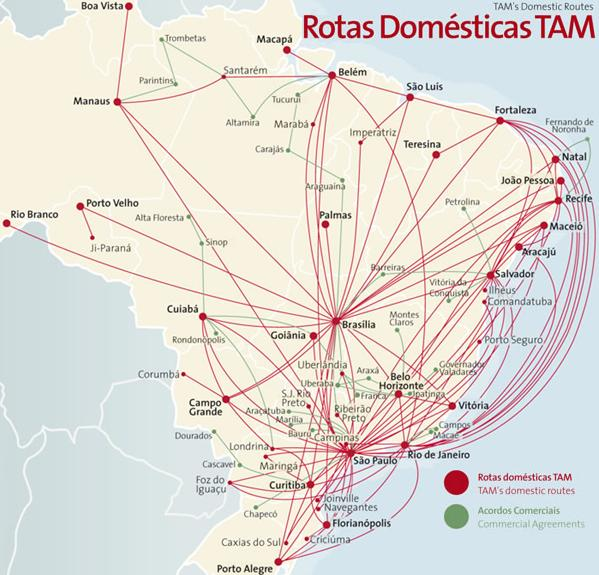
\includegraphics[scale=0.45]{./img/tam_brazilian_airlines}
\end{figure}
	
A malha da Rio Sul se refere a uma instância com voos de um dia de operação da
empresa contendo 107 voos, onde na prática era operado com 20 trilhos
obtidos pela montagem manual de um experiente operador \cite{pontes2002}. A
malha da TAM, que foi obtida manualmente, é formada por 241 voos possuindo
uma grande quantidade de ligações entre os 31 aeroportos envolvidos, dessa
forma essa instância  obteve um maior grau de complexidade.

Essas instâncias foram estendidas para o período de uma semana para testar o
comportamento do algoritmo e do solver, onde a instância da Rio Sul
estendida apresentou 749 voos e a da Tam estendida ficou com 1687 voos.
	
Levou-se em consideração apenas instâncias de companhias aéreas brasileiras pois
as grandes empresas globais apresentam uma malha com característica
\textit{hub-and-spoke}, como pode ser visto na Figura \ref{fig:hubandspoke}. Uma
malha é caracterizada como sendo do tipo \textit{hub-and-spoke} se ela
apresentar uma grande concen tração de voos em poucos aeroportos e
adicionalmente se um voo tem ligação com um \textit{hub} ele não poderá ter
ligação com outros \textit{hubs} a não ser que ele também seja um \textit{hub}.
Instâncias com essa caractéristicas são mais fáceis de serem resolvidas pois
não apresentam a caractéristica explosiva no nível presente nas malhas aéreas brasileiras.
	
\begin{figure}[ht]
\caption{Malha hub-and-spoke. \newline \mbox{Fonte: (Própria)}}
\label{fig:hubandspoke}
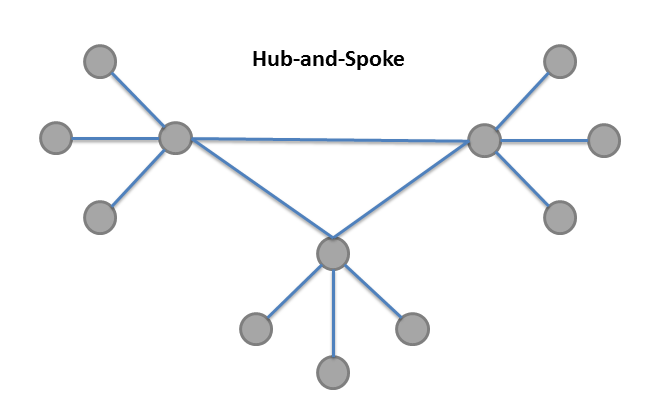
\includegraphics[scale=0.35]{./img/hubandspoke}
\end{figure}
 	 	
	
Não foi possível obter mais instâncias reais pois a comunicação entre essas
empresas e a acadêmia é fraca. Grande parte dessa falta de comunicação se deve
ao receio de revelar dados que podem vir a lhes prejudicar junto a concorrência.

As instâncias podem ser vistas nos anexos ao final desse trabalho.


\section {Objetivos do trabalho}

% Falar das consequências dos objetivos (em termo de economia e em relação a
% melhora do trafego aereo, no brasil, pois irá fazer com que as aeronáves
% fiquem mais tempo voando. O principal problema hoje é na falta de espaço no
% solo para pousar os avioes.

\subsection{Geral}
Tendo em vista os aspectos apresentados, o objetivo principal dessa dissertação
consiste no desenvolvimento de um método híbrido baseado nas metaheurísticas
GRASP e ILS e em programação linear inteira para a resolução do problema
construção de trilhos de aeronaves (PCTA) cobrindo todos os voos planejados com
o menor número de aeronaves bem como efetuando a menor mudança possível no
planejamento inicial desses voos. 

\subsection{Específicos}

Esse trabalho também visa a disponibilização de um conjunto de instâncias com
os resultados que foram obtidos. Isso irá permitir a sua comparação com
outros trabalhos no futuro.

O método proposto consegue acelerar a convergência da fase de busca local
através de uma busca exata em uma vizinhança restrita usando programação
linear inteira. Adicionalmente esse método permite escapar de minimos locais.

Para conseguir melhores resultados foi permitido, em alguns cenários, a
utilização de pequenas alterações no horário de partida sugerido dos voos bem
como a criação de voos de reposicionamento.

\section {Organização da proposta }

O restante desse trabalho está estruturado da seguinte forma:

\begin{itemize}

\item Capítulo 2: Apresenta a fundamentação sobre otimização, metaheurísticas
e programação linear inteira. A seção referente às metaheurísticas inicia
com uma descrição, seguida do detalhamento das metaheurísticas utilizadas no trabalho,
o GRASP e o ILS.

%Ao final da fundamentação teórica
%será feita uma revisão dos principais trabalhos relacionados ao presente
%trabalho que estão presentes na literatura.

\item Capítulo 3: Descreve o problema, explicando os conceitos que são
utilizados no trabalho.

\item Capítulo 4: Introduz o modelo matemático que foi desenvolvido.

\item Capítulo 5: Descreve o método proposto nesse trabalho, mostrando como foi
feita a integração das metaheurísticas e da programação linear inteira e também descreve os parâmetros e as restrições que foram utilizadas.

\item Capítulo 6: Apresenta os resultados obtidos com o algoritmo e dá
diretrizes de como utilizar o método proposto.
%\item Capítulo 8: Dá uma conclusão, indicando o que tem que ser melhorado e o que se espera ter para a finalização do trabalho.

\item No final é apresentado a bibliográfia e os anexos que contém um maior
detalhamento das instâncias e dos resultados obtidos.

\end{itemize}